\documentclass[border=5pt]{standalone}
\usepackage{tikz}
\usepackage{amsmath,amssymb}
\usepackage{mathptmx}
\usepackage[T1]{fontenc}
\usetikzlibrary{positioning, arrows.meta, fit, calc}

\renewcommand{\familydefault}{\rmdefault}
\newcommand{\sep}[1]{\rule{#1}{0.4pt}}

\begin{document}
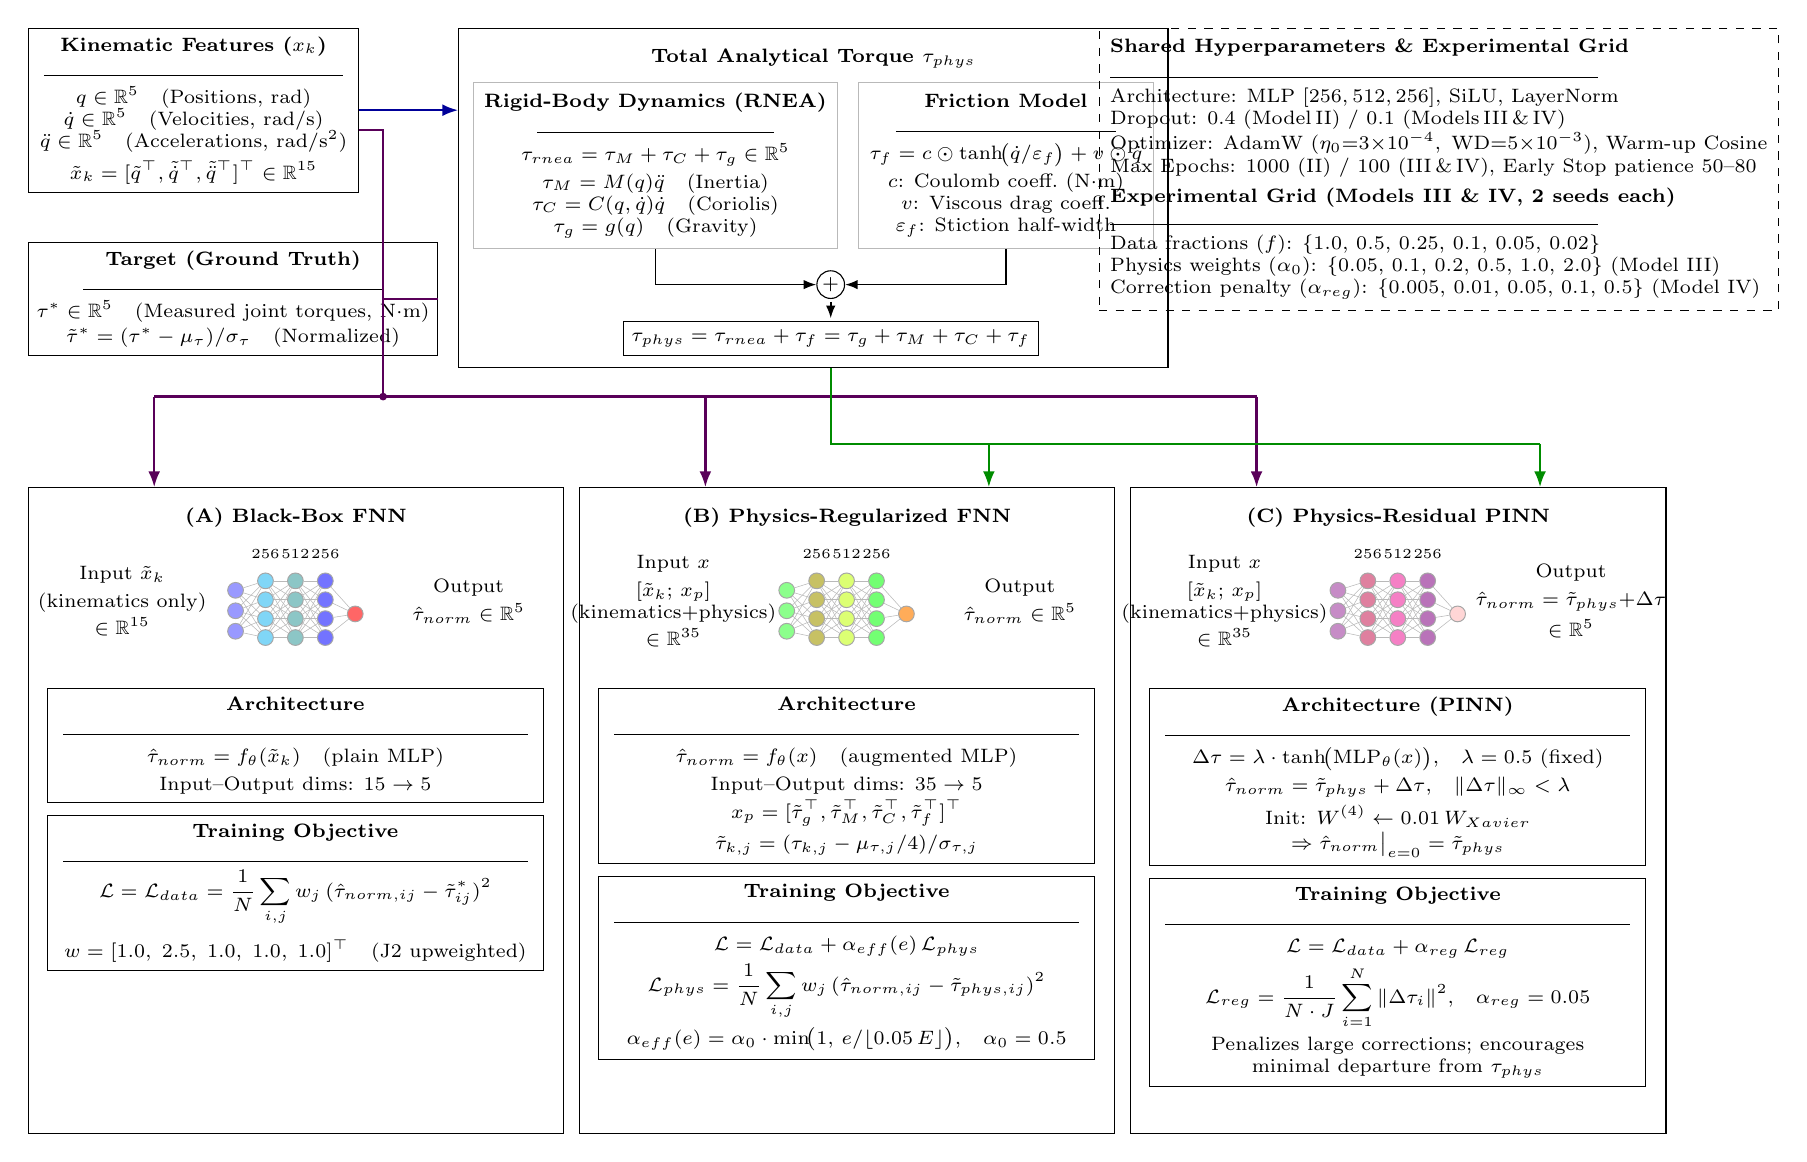
\begin{tikzpicture}[
    font=\scriptsize,
    box/.style={draw, rectangle, align=center, inner sep=3pt},
    subbox/.style={draw=gray!55, align=center, inner sep=4pt},
    arr/.style={-{Latex[length=2mm]}, thick},
    smallarr/.style={-{Latex[length=1.6mm]}, semithick},
    nn/.style={circle, draw=gray!70, line width=0.35pt,
               minimum size=2.0mm, inner sep=0pt}
]

% =========================================================
% Build TOTAL ANALYTICAL TORQUE first
% =========================================================
\node[subbox, anchor=north west] (rbd) at (5.65, -0.45) {
    \textbf{Rigid-Body Dynamics (RNEA)}\\[1pt]
    \sep{3.0cm}\\[2pt]
    $\tau_{rnea}=\tau_M+\tau_C+\tau_g \in \mathbb{R}^{5}$\\[2pt]
    $\tau_M = M(q)\ddot{q}$\quad (Inertia)\\
    $\tau_C = C(q,\dot{q})\dot{q}$\quad (Coriolis)\\
    $\tau_g = g(q)$\quad (Gravity)
};

\node[subbox, anchor=north west, right=0.25cm of rbd] (fric) {
    \textbf{Friction Model}\\[1pt]
    \sep{2.8cm}\\[2pt]
    $\tau_f=c\odot\tanh\!\bigl(\dot{q}/\varepsilon_f\bigr)+v\odot\dot{q}$\\[2pt]
    $c$: Coulomb coeff.\ (N$\cdot$m)\\
    $v$: Viscous drag coeff.\\
    $\varepsilon_f$: Stiction half-width
};

\node[anchor=south, font=\scriptsize\bfseries]
    (tatTitle) at ($(rbd.north west)!0.5!(fric.north east)+(0,0.05)$)
    {Total Analytical Torque $\tau_{phys}$};

\node[circle, draw, inner sep=0.7pt]
    (sum) at ($(rbd.south)!0.5!(fric.south)+(0,-0.45)$) {\scriptsize $+$};

\node[box, below=0.28cm of sum] (tphys)
    {$\tau_{phys}=\tau_{rnea}+\tau_f=\tau_g+\tau_M+\tau_C+\tau_f$};

\draw[smallarr] (rbd.south) |- (sum.west);
\draw[smallarr] (fric.south) |- (sum.east);
\draw[smallarr, shorten <=1pt, shorten >=1pt] (sum.south) -- (tphys.north);

\node[draw, fit=(tatTitle)(rbd)(fric)(tphys),
      inner xsep=5pt, inner ysep=4pt] (tat) {};

% =========================================================
% KIN and HYPER aligned to tat.north
% =========================================================
\path let \p1=(tat.north) in coordinate (kinAnchor)   at (0,    \y1);
\path let \p1=(tat.north) in coordinate (hyperAnchor) at (13.6, \y1);

\node[box, anchor=north west, minimum width=4.2cm] (kin) at (kinAnchor) {
    \textbf{Kinematic Features ($x_k$)}\\[1pt]
    \sep{3.8cm}\\[2pt]
    $q \in \mathbb{R}^{5}$\quad (Positions, rad)\\
    $\dot{q} \in \mathbb{R}^{5}$\quad (Velocities, rad/s)\\
    $\ddot{q} \in \mathbb{R}^{5}$\quad (Accelerations, rad/s$^2$)\\[2pt]
    $\tilde{x}_k = [\tilde{q}^\top,\tilde{\dot{q}}^\top,\tilde{\ddot{q}}^\top]^\top \in\mathbb{R}^{15}$
};

\node[draw, dashed, align=left, inner sep=4pt, anchor=north west,
    minimum width=6.5cm] (hyper) at (hyperAnchor) {
    \textbf{Shared Hyperparameters \& Experimental Grid}\\[1pt]
    \sep{6.2cm}\\[1pt]
    Architecture: MLP $[256, 512, 256]$, SiLU, LayerNorm\\
    Dropout: 0.4 (Model\,II) / 0.1 (Models\,III\,\&\,IV)\\
    Optimizer: AdamW $(\eta_0{=}3{\times}10^{-4},\;\text{WD}{=}5{\times}10^{-3})$, Warm-up Cosine\\
    Max Epochs: 1000 (II) / 100 (III\,\&\,IV), Early Stop patience 50--80\\[3pt]
    \textbf{Experimental Grid (Models III \& IV, 2 seeds each)}\\
    \sep{6.2cm}\\[1pt]
    Data fractions ($f$): $\{1.0,\,0.5,\,0.25,\,0.1,\,0.05,\,0.02\}$\\
    Physics weights ($\alpha_0$): $\{0.05,\,0.1,\,0.2,\,0.5,\,1.0,\,2.0\}$ (Model III)\\
    Correction penalty ($\alpha_{reg}$): $\{0.005,\,0.01,\,0.05,\,0.1,\,0.5\}$ (Model IV)
};

\node[box, anchor=south west, minimum width=4.2cm]
    (target) at (kin.south west |- tphys.south) {
    \textbf{Target (Ground Truth)}\\[1pt]
    \sep{3.8cm}\\[2pt]
    $\tau^* \in\mathbb{R}^{5}$\quad(Measured joint torques, N$\cdot$m)\\[1pt]
    $\tilde{\tau}^* = (\tau^*-\mu_\tau)/\sigma_\tau$\quad(Normalized)
};

% =========================================================
% Neural network macro
% =========================================================
\def\drawNN#1#2#3#4#5#6#7#8{%
    \foreach \i in {1,2,3} \node[nn, fill=#4] (#1i\i) at (#2+0.0,#3+0.40-0.26*\i) {};
    \foreach \i in {1,...,4} \node[nn, fill=#5] (#1a\i) at (#2+0.38,#3+0.50-0.24*\i) {};
    \foreach \i in {1,...,4} \node[nn, fill=#6] (#1b\i) at (#2+0.76,#3+0.50-0.24*\i) {};
    \foreach \i in {1,...,4} \node[nn, fill=#7] (#1c\i) at (#2+1.14,#3+0.50-0.24*\i) {};
    \node[nn, fill=#8] (#1o) at (#2+1.52,#3-0.16) {};
    \foreach \i in {1,2,3} \foreach \j in {1,...,4} \draw[gray!55,line width=0.2pt] (#1i\i)--(#1a\j);
    \foreach \i in {1,...,4} \foreach \j in {1,...,4} \draw[gray!55,line width=0.2pt] (#1a\i)--(#1b\j);
    \foreach \i in {1,...,4} \foreach \j in {1,...,4} \draw[gray!55,line width=0.2pt] (#1b\i)--(#1c\j);
    \foreach \i in {1,...,4} \draw[gray!55,line width=0.2pt] (#1c\i)--(#1o);
}

% =========================================================
% PANELS  -- panel height increased so loss boxes stay inside
% =========================================================
\def\panelW{6.8}
\def\panelH{8.2}        % increased from 6.7 -> 8.2 to fully contain loss boxes
\def\panelY{-5.6}
\def\panelShiftB{7.0}
\def\panelShiftC{14.0}

\def\dataBusY{-4.45}
\def\physBusY{-5.05}

\def\inX{1.2}
\def\nnX{2.64}
\def\outX{5.6}
\def\ioY{-1.45}
\def\archY{-2.55}       % top of Architecture box -- right under NN
\def\archX{3.4}
\def\boxW{6.3}

\tikzset{
    panelTitle/.style={anchor=north, font=\scriptsize\bfseries},
    io/.style={align=center, font=\scriptsize}
}

% ---------- Panel A: Black Box ----------
\begin{scope}[shift={(0, \panelY)}]
    \node[draw, minimum width=\panelW cm, minimum height=\panelH cm,
        anchor=north west] (Apanel) at (0,0) {};
    \node[panelTitle] at ([yshift=-4pt]Apanel.north)
        {(A) Black-Box FNN};

    \node[io] at (\inX,\ioY) {Input $\tilde{x}_k$\\[2pt](kinematics only)\\[2pt]$\in\mathbb{R}^{15}$};
    \drawNN{A}{\nnX}{\ioY}{blue!40}{cyan!50}{teal!45}{blue!55}{red!60}
    \node[font=\tiny, above=0.05cm of Aa1] {256};
    \node[font=\tiny, above=0.05cm of Ab1] {512};
    \node[font=\tiny, above=0.05cm of Ac1] {256};
    \node[io] at (\outX,\ioY) {Output\\[2pt]$\hat{\tau}_{norm}\in\mathbb{R}^{5}$};

    \node[box, minimum width=\boxW cm, anchor=north] (Aarch) at (\archX,\archY) {
        \textbf{Architecture}\\[1pt]\sep{5.9cm}\\[2pt]
        $\hat{\tau}_{norm} = f_\theta(\tilde{x}_k)$\quad (plain MLP)\\[2pt]
        Input--Output dims: $15 \to 5$
    };
    \node[box, minimum width=\boxW cm, below=0.15cm of Aarch] (Aloss) {
        \textbf{Training Objective}\\[1pt]\sep{5.9cm}\\[2pt]
        $\mathcal{L} = \mathcal{L}_{data} = \dfrac{1}{N}\displaystyle\sum_{i,j} w_j\,(\hat{\tau}_{norm,ij} - \tilde{\tau}^*_{ij})^2$\\[4pt]
        $w = [1.0,\;2.5,\;1.0,\;1.0,\;1.0]^\top$\quad (J2 upweighted)
    };
\end{scope}

% ---------- Panel B: Physics Regularized ----------
\begin{scope}[shift={(\panelShiftB, \panelY)}]
    \node[draw, minimum width=\panelW cm, minimum height=\panelH cm,
        anchor=north west] (Bpanel) at (0,0) {};
    \node[panelTitle] at ([yshift=-4pt]Bpanel.north)
        {(B) Physics-Regularized FNN};

    \node[io] at (\inX,\ioY) {Input $x$\\[2pt]$[\tilde{x}_k;\, x_p]$\\(kinematics+physics)\\[2pt]$\in\mathbb{R}^{35}$};
    \drawNN{B}{\nnX}{\ioY}{green!45}{olive!50}{lime!55}{green!55}{orange!65}
    \node[font=\tiny, above=0.05cm of Ba1] {256};
    \node[font=\tiny, above=0.05cm of Bb1] {512};
    \node[font=\tiny, above=0.05cm of Bc1] {256};
    \node[io] at (\outX,\ioY) {Output\\[2pt]$\hat{\tau}_{norm}\in\mathbb{R}^{5}$};

    \node[box, minimum width=\boxW cm, anchor=north] (Barch) at (\archX,\archY) {
        \textbf{Architecture}\\[1pt]\sep{5.9cm}\\[2pt]
        $\hat{\tau}_{norm} = f_\theta(x)$\quad (augmented MLP)\\[2pt]
        Input--Output dims: $35 \to 5$\\[2pt]
        $x_p = [\tilde{\tau}_g^\top,\tilde{\tau}_M^\top,\tilde{\tau}_C^\top,\tilde{\tau}_f^\top]^\top$\\[2pt]
        $\tilde{\tau}_{k,j} = (\tau_{k,j} - \mu_{\tau,j}/4)/\sigma_{\tau,j}$
    };
    \node[box, minimum width=\boxW cm, below=0.15cm of Barch] (Bloss) {
        \textbf{Training Objective}\\[1pt]\sep{5.9cm}\\[2pt]
        $\mathcal{L} = \mathcal{L}_{data} + \alpha_{eff}(e)\,\mathcal{L}_{phys}$\\[2pt]
        $\mathcal{L}_{phys} = \dfrac{1}{N}\displaystyle\sum_{i,j} w_j\,(\hat{\tau}_{norm,ij} - \tilde{\tau}_{phys,ij})^2$\\[2pt]
        $\alpha_{eff}(e) = \alpha_0 \cdot \min\!\bigl(1,\, e / \lfloor 0.05\,E\rfloor\bigr)$,\quad $\alpha_0=0.5$
    };
\end{scope}

% ---------- Panel C: Physics Residual (PINN) ----------
\begin{scope}[shift={(\panelShiftC, \panelY)}]
    \node[draw, minimum width=\panelW cm, minimum height=\panelH cm,
        anchor=north west] (Cpanel) at (0,0) {};
    \node[panelTitle] at ([yshift=-4pt]Cpanel.north)
        {(C) Physics-Residual PINN};

    \node[io] at (\inX,\ioY) {Input $x$\\[2pt]$[\tilde{x}_k;\, x_p]$\\(kinematics+physics)\\[2pt]$\in\mathbb{R}^{35}$};
    \drawNN{C}{\nnX}{\ioY}{violet!45}{purple!50}{magenta!50}{violet!55}{pink!65}
    \node[font=\tiny, above=0.05cm of Ca1] {256};
    \node[font=\tiny, above=0.05cm of Cb1] {512};
    \node[font=\tiny, above=0.05cm of Cc1] {256};
    \node[io] at (\outX,\ioY) {Output\\[2pt]$\hat{\tau}_{norm}=\tilde{\tau}_{phys}{+}\Delta\tau$\\[2pt]$\in\mathbb{R}^{5}$};

    \node[box, minimum width=\boxW cm, anchor=north] (Carch) at (\archX,\archY) {
        \textbf{Architecture (PINN)}\\[1pt]\sep{5.9cm}\\[2pt]
        $\Delta\tau = \lambda\cdot\tanh\!\bigl(\text{MLP}_\theta(x)\bigr)$,\quad $\lambda=0.5$ (fixed)\\[2pt]
        $\hat{\tau}_{norm} = \tilde{\tau}_{phys} + \Delta\tau$,\quad $\|\Delta\tau\|_\infty < \lambda$\\[2pt]
        Init: $W^{(4)} \leftarrow 0.01\,W_{Xavier}$\\[1pt]
        $\Rightarrow \hat{\tau}_{norm}\big|_{e=0} = \tilde{\tau}_{phys}$
    };
    \node[box, minimum width=\boxW cm, below=0.15cm of Carch] (Closs) {
        \textbf{Training Objective}\\[1pt]\sep{5.9cm}\\[2pt]
        $\mathcal{L} = \mathcal{L}_{data} + \alpha_{reg}\,\mathcal{L}_{reg}$\\[2pt]
        $\mathcal{L}_{reg} = \dfrac{1}{N \cdot J}\displaystyle\sum_{i=1}^{N}\|\Delta\tau_i\|^2$,\quad $\alpha_{reg}=0.05$\\[2pt]
        Penalizes large corrections; encourages\\
        minimal departure from $\tau_{phys}$
    };
\end{scope}

% =========================================================
% ARROWS
% =========================================================

\draw[arr, blue!60!black] (kin.east) -- (tat.west |- kin.east);

\coordinate (busA) at ($(Apanel.north)+(-1.8,0)$);
\coordinate (busB) at ($(Bpanel.north)+(-1.8,0)$);
\coordinate (busC) at ($(Cpanel.north)+(-1.8,0)$);

\draw[violet!70!black, thick]
    (busA |- 0,\dataBusY) -- (busC |- 0,\dataBusY);

\coordinate (kinExit) at ($(kin.east)+(0,-0.25)$);
\draw[violet!70!black, thick]
    (kinExit) -- ++(0.30,0) coordinate (kinJog)
    -- (kinJog |- 0,\dataBusY);

\coordinate (targetExit) at (target.east);
\draw[violet!70!black, thick]
    (targetExit) -- (kinJog |- targetExit)
    -- (kinJog |- 0,\dataBusY);

\fill[violet!70!black] (kinJog |- 0,\dataBusY) circle (1.4pt);

\draw[arr, violet!70!black] (busA |- 0,\dataBusY) -- (busA);
\draw[arr, violet!70!black] (busB |- 0,\dataBusY) -- (busB);
\draw[arr, violet!70!black] (busC |- 0,\dataBusY) -- (busC);

\coordinate (tphysExit) at (tphys.south |- tat.south);
\coordinate (physB) at ($(Bpanel.north)+(1.8,0)$);
\coordinate (physC) at ($(Cpanel.north)+(1.8,0)$);

\draw[green!55!black, thick]
    (tphysExit) -- (tphysExit |- 0,\physBusY)
    -- (physC |- 0,\physBusY);

\draw[arr, green!55!black] (physB |- 0,\physBusY) -- (physB);
\draw[arr, green!55!black] (physC |- 0,\physBusY) -- (physC);

\end{tikzpicture}
\end{document}